% thieu: Tensorlfow-Converter

\section{Model deployment}
The thesis introduced a few CNNs developed for mobile devices; the Android platform and accompanied libraries were also indicated. The thesis will give an overall view of ML models deployment on both servers and mobile phones in the section below. 

\subsection{Deployment on Server/Cloud Platforms}
Some frameworks (e.g., Tensorflow Serving, Triton) and platforms (e.g., Google Cloud ML Engine, Amazon SageMaker) can facilitate this deployment. The following figure illustrates how to serve deep learning models on cloud/server.

\begin{figure} [H]
    \centering
    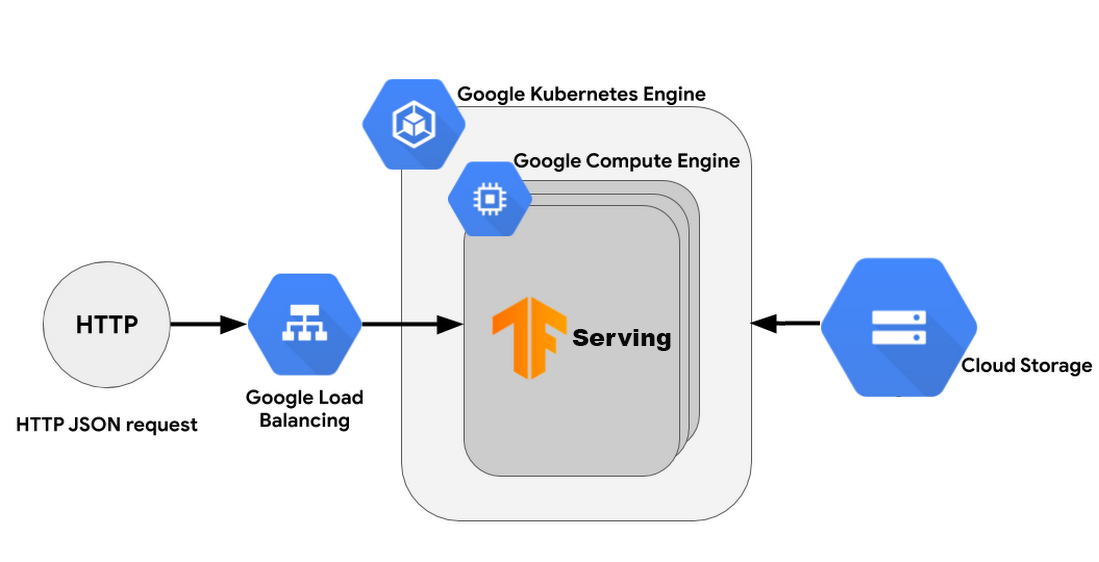
\includegraphics[width=0.9\textwidth]{chapter2/image/tfserving.png}
    \caption{Model deployment on Google Cloud}
    \label{fig:cloud}
\end{figure}

\paragraph{TF Serving}
TF Serving \cite{tfserving} is a deep learning framework specially designed to deploy deep learning models to servers. It operates as a set of processes on one or more network servers, using one of several advanced architectures to handle synchronization and distributed computation. To communicate with TF Model Server, clients are allowed to send inputs and receive outputs through REST or gRPC interfaces. \par 
\paragraph{Google Cloud ML Engine}
Google Cloud ML Engine \cite{googlecloudml} is a popular cloud platform for deploying deep learning software and training deep learning models. To deploy a trained model, the first step is to upload your saved model to a Cloud Storage bucket. After that, TF Serving , installed on all virtual machines in that cluster, loads the model to memory, executes it, and responds to clients. Other more convenient ways to deploy ML models provided by Google are Cloud Functions \cite{cloudfunctions}, and AI Platform Predictions \cite{platformprediction}.
These solutions assist the deployment of your models at scale to get predictions from the cloud, which hosts your model for online and batch prediction requests. \par
%warm invoke


\subsection{Deployment on Mobile Platforms}
In this section, the thesis talks about the deployment of ML models on smartphones through introducing the TFLite framework. Firstly, we start with some basic information about this framework. After that, we get a brief view of optimization and adaptation techniques that this framework provides to convert models for on-device inference. \par
\subsubsection{Tensorflow and TFLite}
Tensorflow is the name of a well-known deep learning framework. It is debuted at Google I/O Conference in 2016 as an opensource. After that, it has received goods feedbacks from developer community for its computational supportability and flexible uses for both research and industry. \par

Following the success, Tflite was adapted as a software stack specifically for mobile development in May 2017. Until now, it becomes prevalent and supports both two main mobile OS: iOS and Android. With this comprehensive framework, developing and training new networks for machine learning tasks has become increasingly more reasonable. \par

Both Tensorflow and TFlite are open-source and cross-platform; hence developers are free to clone the source code from Github and build it manually with Bazel afterward. For that, any modifications to operators, targeted architecture, etc., are permissible. This is two commands used to build TFLite: \par

\begin{verbatim}
bazel build -s -c opt --strip always --cxxopt='--std=c++11'
--config=android_arm64 //tensorflow/lite:libtensorflowlite.so

bazel build -s -c opt --strip always --cxxopt='--std=c++11' 
--config android_arm64 //tensorflow/lite/delegates/gpu:
libtensorflowlite_gpu_delegate.so    
\end{verbatim}


All of the above commands are used to build the TFLite library for $arm64-v8a$. The difference is that the first one is to build a shared library for the CPU backend, while the second one is for the GPU backend. In fact, Tflite supports almost major architecture, such as: $armabi$, $armabi-v7a$, $x86$, $x86\_64$. One other benefit of TFLite is that it is compatible with multiple hardware, such as EdgeTPU, NNAPI,  GPU, CPU. \par

\subsubsection{TFLite Converter}\label{subsec:converter}

TFLite Converter is a built-in module, already included in the TFlite framework, executing conversion to light-weight models for edge devices. The converter inputs TensorFlow models and outputs an efficient form for use by the interpreter. In more detail, the converter optimizes the model and then converts to a FlatBuffer, an efficient storage format which can be read later using the TFLite Interpreter on mobile devices. \par

\begin{figure}[H]
    \centering
    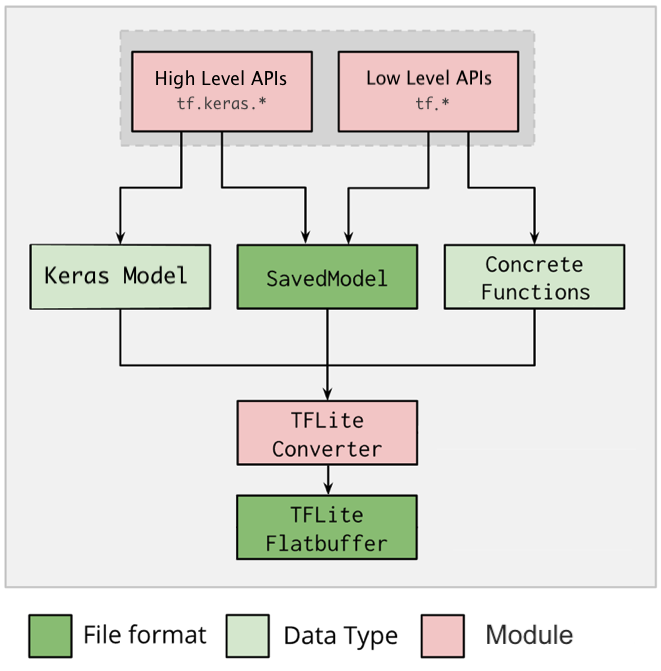
\includegraphics[width=0.6\textwidth]{chapter2/image/tflite3.png}
    \caption{Workflow of TFLite Converter}
    \label{fig:tflite}
\end{figure}
 
The above figure shows steps to convert a Tensorflow model to a TFLite model. As you can see, TFLite Converter only supports several specific saved model formats, which will be listed later. In addition, unsupported and un-predefined operations also cause critical errors, so these must be written in C++ code using Tensorflow C++ API or discarded from the model, so in order to use converter, we need to meet all requirement of input format and architecture.\par 

In relevant to input format requirements, TFLite Converter only supports conversion for three types of data: Keras Model (*.h5), SavedModel (a directory), and Concrete Functions (source code). If you use the version 1, you have additional options: GraphDef from a session or Frozen GraphDef from a file) However, it is deprecated in the version 2 and would not be introduced here. Furthermore, TFlite has restrictions in data type; data of unsupported data type must be cast to a supported one. The prescribed data types are Float32, Int32, Int64, and unsigned Int8. \par


\subsubsection{Quantization} \label{subsec:quantization}
Quantization is one of a few model optimization techniques that is usually used during the conversion of a Tensorflow to a TFLite model. Technically, quantization is the process of assigning values from a large set to values in a smaller set, used here as a technic to change data types. Take conversion from \emph{float32} to \emph{float16} for an example, quantization here is referred to as reducing the precision of a model’s weights; consequently, the memory required to store a parameter is 2 bytes instead of 4 bytes. Hardware support for \emph{int8} computations is typically 2 to 4 times faster when compared to for \emph{float32} computations. Additionally, as there are less data to transport, processors can execute operations with less precise numbers much faster. \par

Quantization can be integrated into training (called quantization aware training) or the post-training phase. More various, models are flexible to only be quantized on weights only or both weights and activations. The following is the equation of a general one: \par

\begin{equation}
    output = (input - min\_range) * \frac{range(data\_type)}{(max\_range - min\_range)}
\end{equation}
Where \begin{itemize}
    \item [$-$] $input$: Value is about to be quantized
    \item [$-$] $min\_range$: Minimum value in the range of input
    \item [$-$] $max\_range$: Maximum value in the range of input
    \item [$-$] $range(data\_type)$: Equals to $max(data\_type) - min(data\_type)$
    \item [$-$] $output$: Value after being quantized
\end{itemize} 

Assume the data type is \emph{float} and has a possible range of [0.0, 10.0] and the quantized data type has an \emph{uint8} range of [0, 255]. In this case, quantizing from \emph{float} to \emph{uint8} will multiply each value by 255/8 and cast to \emph{uint8}. \par

Although quantization is efficient to make the neural networks faster and smaller, this optimization can potentially result in a slight reduction in accuracy, which must be considered during development process. Besides quantization, TFLite Converter provides other powerful optimization techniques, taking weigh pruning and weight clustering for example. They are not introduced in this thesis, though. \par

